% $File: report.tex
% $Date: Mon Oct 28 10:29:29 2013 +0800
% $Author: wyx <ppwwyyxxc@gmail.com>

\documentclass[11pt,a4paper]{article}
\usepackage{fontspec,amsmath,amssymb,zhspacing,verbatim,minted,listings,zhmath}
\usepackage{titlesec, titletoc}
\usepackage{enumerate}
\usepackage[hyperfootnotes=false,colorlinks,linkcolor=blue,anchorcolor=blue,citecolor=blue]{hyperref}
\usepackage{indentfirst}
\usepackage{float}			% don't automatically change location of figure [H]
\usepackage{chngpage}		% use \changetext to change page size
\usepackage{caption}\captionsetup{hypcap=true}  % ref to jump to object instead of caption
\newfontfamily\zhfont[BoldFont=SimHei,ItalicFont=KaiTi_GB2312]{SimSun}
\lstset{keywordstyle=\color{blue!70}, commentstyle=\color{red!50!green!50!blue!50},frame=shadowbox,rulesepcolor=\color{red!20!green!20!blue!20},
basicstyle=\footnotesize\ttfamily}
\zhspacing
\setlength{\parindent}{2em}

\usepackage{fancyhdr}
\changetext{}{2.2cm}{-1.1cm}{-1.1cm}{}
\pagestyle{fancy}
\setlength{\headheight}{15.2pt}
\lhead[]{}\rhead[]{}
\fancyhead[C]{\emph{ALU实验}}


%use cell in tabular
\newcommand{\tabincell}[2]{\begin{tabular}{@{}#1@{}}#2\end{tabular}}

%thick shline
\newlength\savewidth
\newcommand\shline{\noalign{\global\savewidth\arrayrulewidth\global\arrayrulewidth 1pt}
                   \hline
                   \noalign{\global\arrayrulewidth\savewidth}}


\renewcommand{\abstractname}{摘要}
\renewcommand{\contentsname}{目录}
\renewcommand{\tablename}{表}
\renewcommand{\figurename}{图}
\newcommand{\figref}[1]{\hyperref[fig:#1]{图\ref*{fig:#1}}}
\newcommand{\secref}[1]{\hyperref[sec:#1]{\ref*{sec:#1}节}}
\newcommand{\tabref}[1]{\hyperref[tab:#1]{表\ref*{tab:#1}}}

% $File: mint-defs.tex
% $Date: Mon Oct 07 22:04:16 2013 +0800
% $Author: wyx <ppwwyyxxc@gmail.com>


% \inputmintedConfigured[additional minted options]{lang}{file path}{
\newcommand{\inputmintedConfigured}[3][]{\inputminted[fontsize=\footnotesize,
	label=#3,linenos,frame=lines,framesep=0.8em,tabsize=4,#1]{#2}{#3}}

% \phpsrc[additional minted options]{file path}: show highlighted php source
\newcommand{\phpsrc}[2][]{\inputmintedConfigured[#1]{php}{#2}}
% \phpsrcpart[additional minted options]{file path}{first line}{last line}: show part of highlighted php source
\newcommand{\phpsrcpart}[4][]{\phpsrc[firstline=#3,firstnumber=#3,lastline=#4,#1]{#2}}
% \phpsrceg{example id}
\newcommand{\phpeg}[1]{\inputminted[startinline,
	firstline=2,lastline=2]{php}{res/php-src-eg/#1.php}}

\newcommand{\txtsrc}[2][]{\inputmintedConfigured[#1]{text}{#2}}
\newcommand{\txtsrcpart}[4][]{\txtsrc[firstline=#3,firstnumber=#3,lastline=#4,#1]{#2}}

\newcommand{\pysrc}[2][]{\inputmintedConfigured[#1]{py}{#2}}
\newcommand{\pysrcpart}[4][]{\pysrc[firstline=#3,firstnumber=#3,lastline=#4,#1]{#2}}

\newcommand{\confsrc}[2][]{\inputmintedConfigured[#1]{squidconf}{#2}}
\newcommand{\confsrcpart}[4][]{\confsrc[firstline=#3,firstnumber=#3,lastline=#4,#1]{#2}}

\newcommand{\cppsrc}[2][]{\inputmintedConfigured[#1]{cpp}{#2}}
\newcommand{\cppsrcpart}[4][]{\cppsrc[firstline=#3,firstnumber=#3,lastline=#4,#1]{#2}}

\newcommand{\matsrc}[2][]{\inputmintedConfigured[#1]{matlab}{#2}}
\newcommand{\matsrcpart}[4][]{\matsrc[firstline=#3,firstnumber=#3,lastline=#4,#1]{#2}}


\title{计算机组成原理Project2 -- ALU实验}
\author{吴育昕~刘啸宇~宋方睿}
\date{}

\begin{document}
%\fontsize{10pt}{\baselineskip}
%\selectfont
\maketitle
\tableofcontents

%\begin{abstract}

	%{\bf 关键词}
%\end{abstract}

\titleformat*{\section}{\centering\Large\bf}

% File: intro.tex
% Date: Fri Dec 13 17:36:18 2013 +0800
% Author: Yuxin Wu <ppwwyyxxc@gmail.com>

\section{实验目的}
\begin{enumerate}
  \item 实现以16位THCO-MIPS指令集为核心的基础计算机系统
  \item 实现CPU的流水线结构
  \item 能够使用串口和PC进行通信.
\end{enumerate}

\section{实验工具及环境}
\begin{description}
  \item[操作系统] Windows XP (虚拟机)
  \item[软件] Xilinx ISE 14.6
  \item[语言] Verilog
\end{description}

\section{实现架构}
我们实现了基于流水的16位THCO-MIPS CPU. 其数据通路架构如下:
\begin{figure}[H]
  \centering
  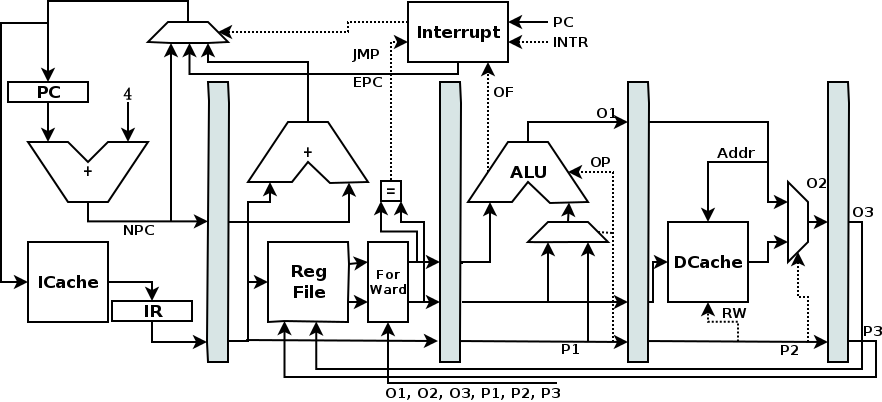
\includegraphics[width=\textwidth]{figure/mips.png}
\end{figure}

\section{模块设计}
整个系统的模块划分较为复杂.其主要模块如下.
\begin{enumerate}
  \item 主板 \verb|motherBoard.v|: 项目顶层模块,包含整个主板,用于链接外部接口.
  \item 中央处理器 \verb|cpu.v|: 包含了CPU的全部逻辑.
  \item RAM控制器 \verb|memory.v|: RAM的封装.
  \item 串口控制器\verb|serialPort.v|: 串口的封装.
  \item 内存映射器 \verb|memoryMapping.v|: 所有外部存储设备通过其与CPU链接.
  \item 显卡 \verb|graphicCard.v|: 渲染CPU内部信号状态,方便调试.
\end{enumerate}

\subsection{CPU模块设计}
  \subsubsection{IF模块}
    本模块主要功能是从存储设备中读取一条指令.
    接受一个PC值做为输入,在前半周期读取其对应的IR,在后半周期将其写入输出IR.
  \subsubsection{ID模块}
    本模块是进行指令的译码,输入为IF阶段读出的指令,输出为三个操作寄存器编号与跳转控制信号.
    前半周期会将IF模块输出的IR缓存,后半周期根据其值输出三个寄存器编号(源寄存器,辅助寄存器与目标寄存器).
    特别注意的是同时会输出跳转控制信号来表明是该指令是否是跳转指令以及其类型.
    源寄存器(register S)同时也被做为跳转判断所需的非T寄存器,辅助寄存器(register M)做为第二操作数或者内存地址基准,目标寄存器(register T)是写回的寄存器编号.
    该阶段能够解析THCO-MIPS指令集的全部44条CPU指令与自己添加的eret指令,见\verb|instructDecoder.v|.
  \subsubsection{EX模块}
    EX模块有ALU与内存地址计算两个子模块.
    ALU子模块将根据转发的指令自己译码,仅接受实际运算型指令,会根据旁路选择出的实际寄存器数据与译码出的立即数进行运算,同时设置T寄存器.
    此外,还将进行内存地址计算,该子模块自己译码,仅接受访存型指令,会根据旁路选择的内存地址基准和译码出的立即数计算出操作内存地址,同时还将输出内存的控制信号.
  \subsubsection{ME模块}
    本模块读入EX模块输出的内存控制信号,进行实际的读入写出操作.该阶段还将从内存读出与EX转发的计算结果中选择一个做为ME阶段的结果输出.
  \subsubsection{WB模块}
    本模块没有单独分模块而是寄存器堆的一部分,将接受一路转发的目标寄存器(register T)的编号与ME模块输出的计算结果,在前半周期进行写入操作.

  \subsubsection{转发器}
    有很多数据在不同模块中均要使用,而且很多很杂.所以设计了转发器,其功能非常单一,即在前半周期读入缓存,后半周期用缓存更新输出.
    根据需要设计了16,4,2和1位的转发器供不同大小的信号使用.实现中共复用8次,节省了大量代码,是核心代码中复用次数最多的模块.
  \subsubsection{PC计算器}
    PC是程序流控制的关键数据,对其修改的方式非常多样,所以专门设计了PC计算器来计算下一个PC值.
    其将接受现在的PC值,跳转指令计算的跳转PC值与中断处理器提供的中断PC,并从中选择一个做为下一个PC值.
    特别的是其将输出一个不考虑中断的情况下的下一个PC做为中断处理后的返回PC值交给中断处理器存储.
  \subsubsection{寄存器堆}
    提供了通用及特殊寄存器的两个读端口和一个写端口,以及T寄存器的一个读端口和一个写端口.
    对通用/特殊寄存器的写入发生在前半周期,以保证译码阶段能够读出正确的寄存器值.
    对T寄存器的写如发生在EX模块拉低T写入使能端时,以保证T寄存器的值为最新.

\subsection{读写分离}
由于每个阶段的输入均是上一阶段的结果,然而在流水作业中,可能某阶段先修改了输出,后一阶段才使用其做为输入.
为了解决这一问题,将每个时钟周期划分为读入半周期和写出半周期.
每一阶段在读入半周期时将上一阶段的输出进行读入缓存,然后在输出半周期内使用缓存下来的数据进行写出.
这样就避免了数据被错误读取的问题.
\subsection{数据旁路}
由于流水线的存在,很多时候上一条指令尚未写回时,下一条指令需要使用其做为源寄存器.
因此从执行阶段和访存阶段引出两条旁路交给译码阶段,如果发现使用的数据被更新但是尚未写回则使用旁路回传的数据而非寄存器堆取出的数据.
旁路会被合并两次,首先是寄存器读出值和上上条指令(执行到ME阶段)的ME输出值进行合并,然后再和上条指令(执行到EX阶段)的EX输出值进行合并.
但是无论如何,如果上一条指令是访存指令写入的值永远不能被迅速转.该情况称之为加载延迟,根据MIPS标准可以交由汇编器处理.
\subsection{跳转}
跳转指令最快可以在译码阶段才能知道其是否跳转,因此会留下一个被允许的延时槽.
为了统一跳转指令的行为以精简设计,我们在译码阶段将是否跳转解析完毕,所有的跳转指令都在译码阶段结束时生效,
因而仅会产生一个延时槽而且不需插入气泡.
\subsection{存储}
CPU可能会访问不同的设备,但是不可能为每一个设备定一条CPU指令,因此所有的外设全部被映射到地址的一部分,
由内存地址映射单元(MMU)来决定对于某内存地址其对应的实际外部设备与其实际物理地址.
这样对任意外存的访问对CPU而言均是一次对内存的访问.实现见\verb|memoryMapping.v|

在RAM的存储上,由于是流水线的架构,其一条指令需要读写内存两次,在内存资源上会产生结构冲突.
注意到实际RAM可以进行连续读取,但不能进行连续写入,因此实现中在同一周期的前半段与后半段将会进行两次操作.
首先进行一次只读操作,然后进行读写操作,可以解决该冲突.
\subsection{显卡}
硬件开发一大难点是仿真结果可能和实际结果不一致,虽然仿真可以检查出一部分错误,但是实际综合后可能出现仿真难以发现的问题.
而在硬件上进行调试不是非常方便,可能需要每次引出不同的信号显示在LED或者数码管上,每次可以监控的信号量有限.
因此在编写核心代码之前实现了一个VGA显示模块,可以显示数字, 字母, 大大方便了调试. 如下图所示:
\begin{figure}[H]
  \centering
  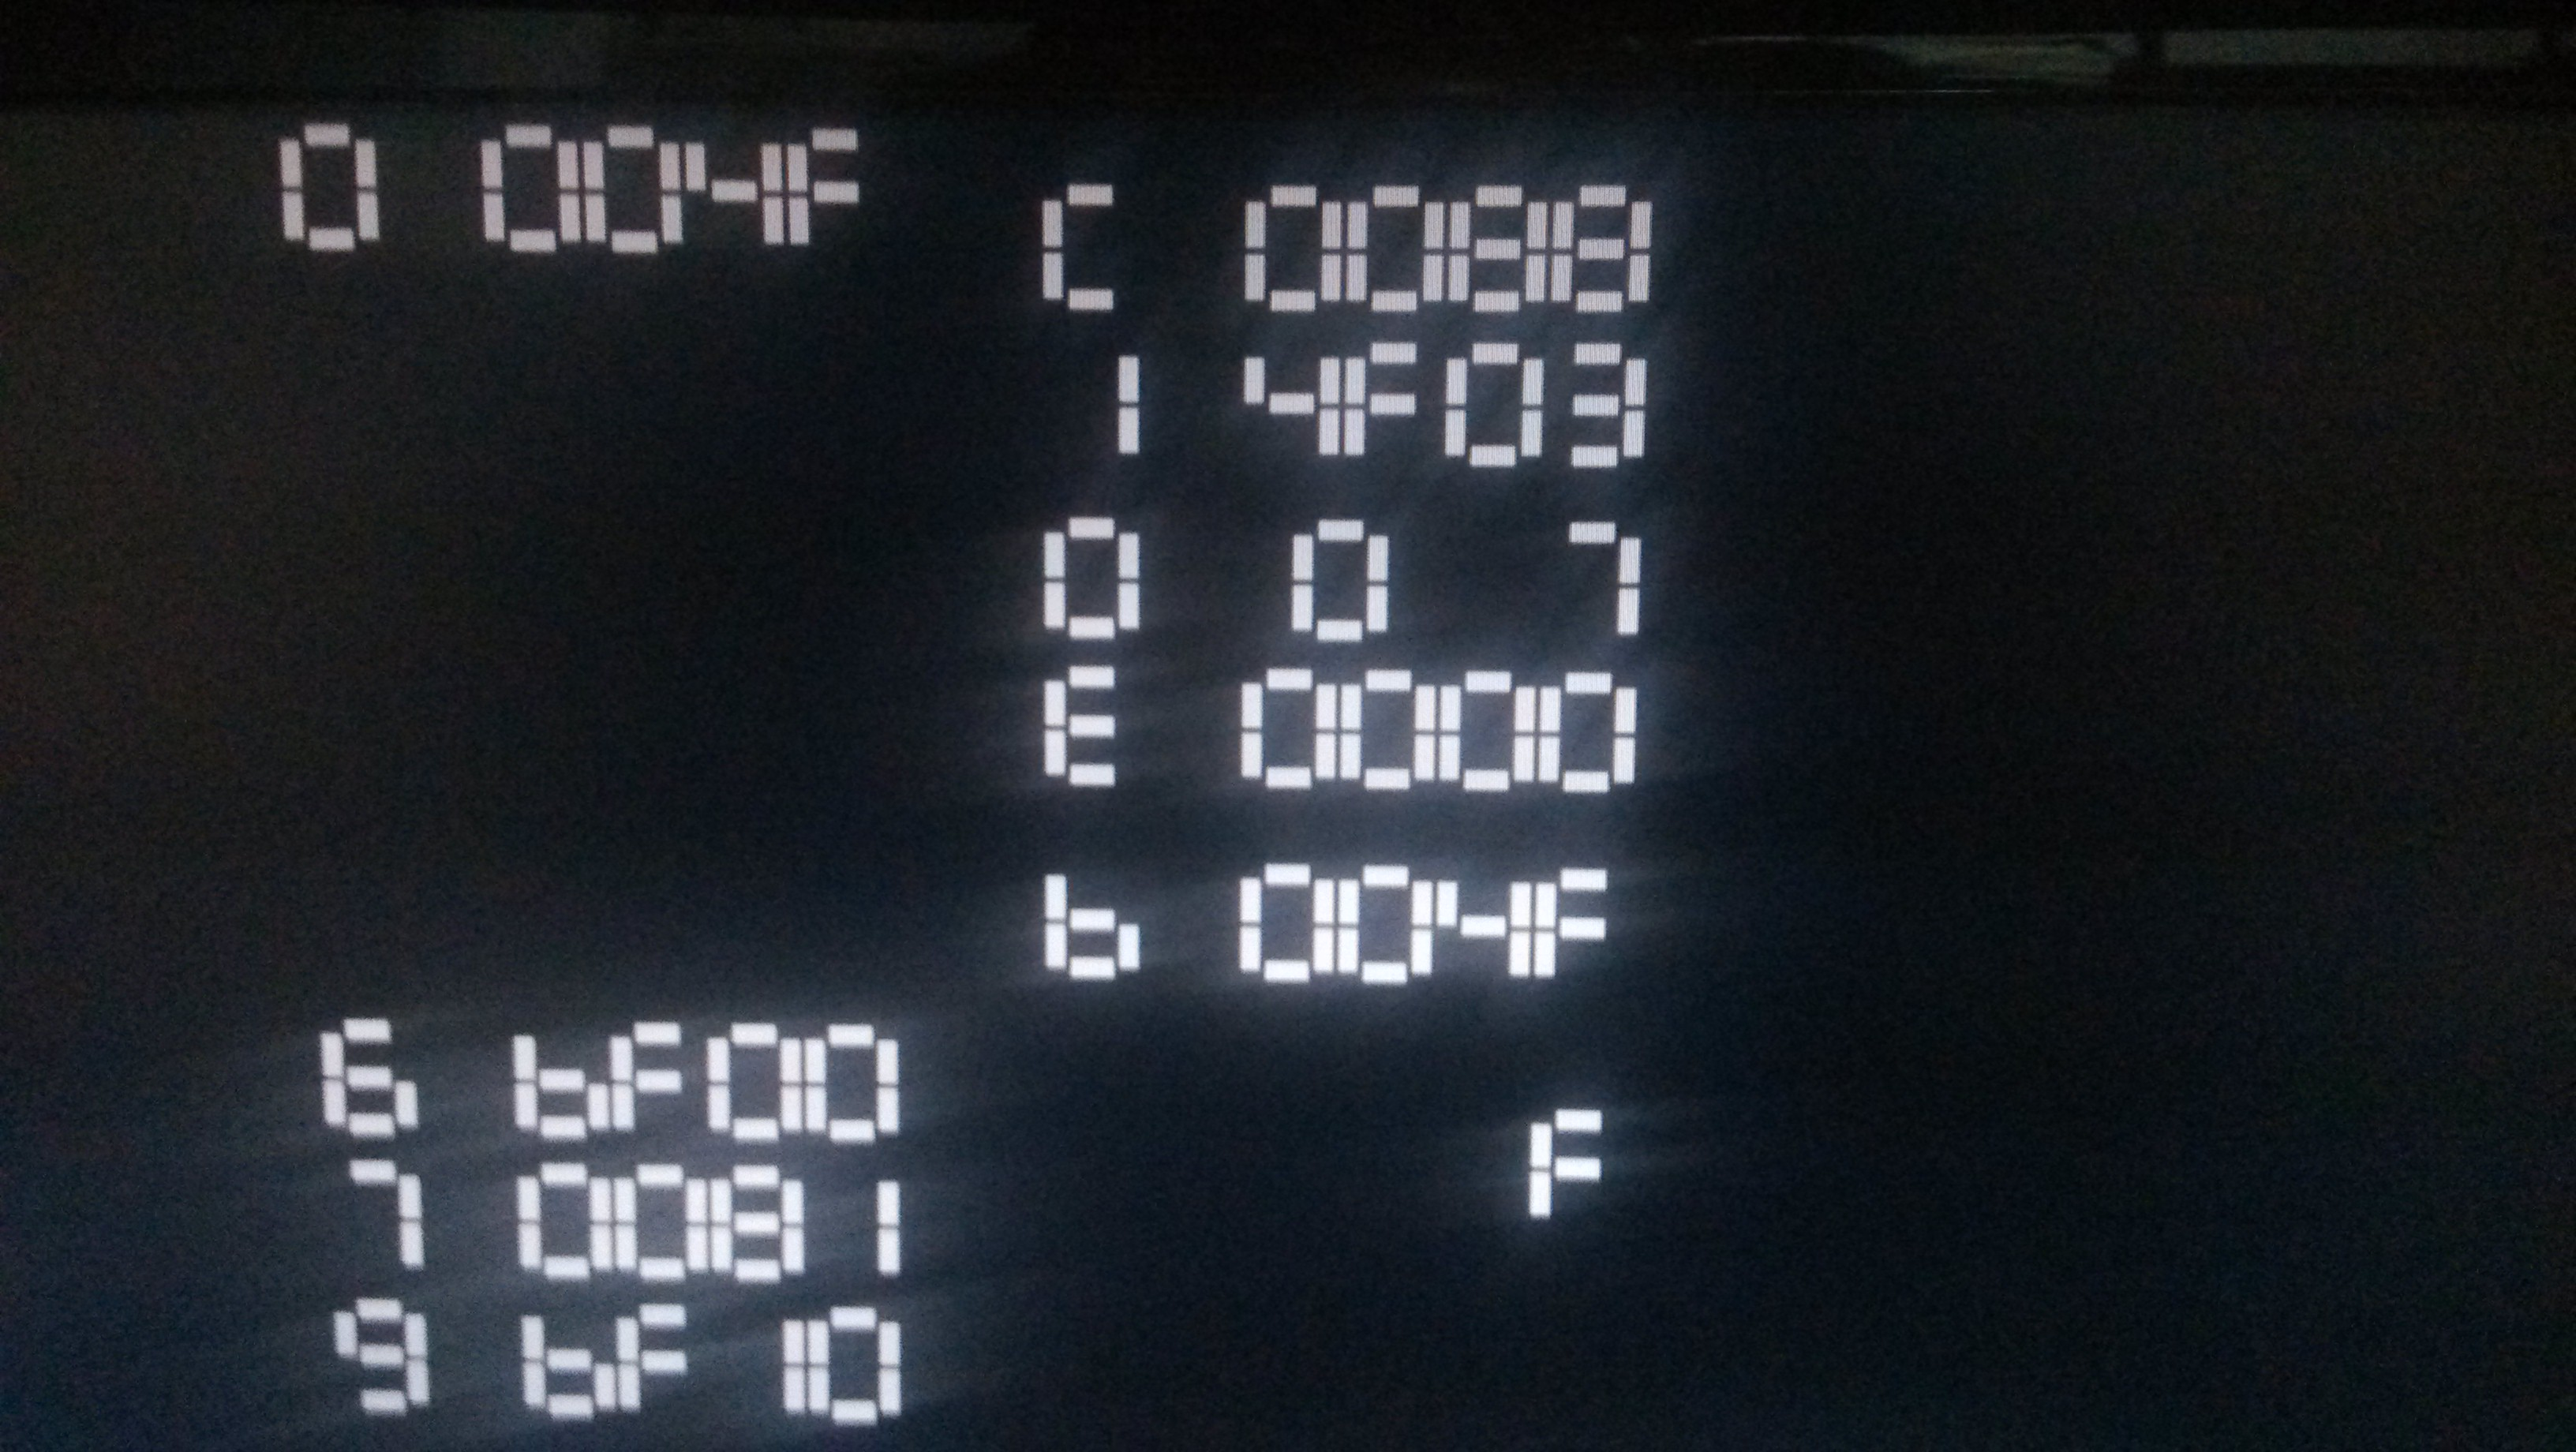
\includegraphics[width=\textwidth]{figure/vga.jpg}
\end{figure}

\subsection{中断}
中断是计算机的一个重要组成部分.为了实现中断,引入了一个新的指令eret,其作用便是从中断处理程序中返回.
中断分为硬中断和软中断,此次作业中将其进行了分级,硬中断的优先级高于软中断.
处理时首先由中断仲裁器决定触发哪一个中断,中断处理器查看是否可以触发中断.
如果可以则会记录当前的PC值与取指令阶段取出的指令,修改PC值为中断处理程序入口,设置中断屏蔽位,并将气泡(nop)传给译码阶段.
在接收到eret指令时,中断处理器将PC还原,恢复中断屏蔽位,并无视取出的指令,把之前存储的指令交给译码阶段继续执行.
因此中断触发int和返回指令eret均无延时槽.
触发中断时引入的气泡也是本项目中唯一可能引入的气泡.

\subsection{汇编器}
在调试中为了测试更多的代码需要写一些复杂的程序.
而给出的汇编器仅仅对汇编指令做了机械的翻译,因此我们用ruby实现了一个支持伪指令的汇编器,见\verb|bin/assembler|.
可以将伪指令如if, else等翻译成CPU指令,语法上也更优美, 减少了编写复杂程序出现的bug的机会. 例如它可以支持如下程序:
\begin{lstlisting}
  main_loop:
  lw r5 r6 0                            # r5 = pos
  lw r4 r7 0                            # r4 = cell[pos]
  li r2 0                               # row of next character
  li r3 0                               # column of next character
  .if r5 == '+'
  addiu r4 1
  sw r7 r4 0
  .elif r5 == '-'
  addiu r4 -1
  sw r7 r4 0
  .elif r5 == '<'
  addiu r7 -1
  .elif r5 == '>'
  addiu r7 1
  .elif r5 == '.'
  move r1 r4
  int 3
  addiu r3 1
  .if r3 == 64
  addiu r2 1
  li r3 0
  .end
  .elif r5 == ','
  # TODO
  .elif r5 == '['
  .if r4 == 0
  xor r3 r3             # number of unmatched parentheses
\end{lstlisting}
\section{实验结果}
最终实现的版本有两个.
\subsection{目标分支}
期望目标是能够运行文本编辑器并在VGA上显示,但是由于硬中断的实现时间太晚,没有足够的时间基于其继续开发,因此只停留在将键盘输入数据载入I/O缓存区的步骤.
\subsection{基础分支}
基础分支实现了串口,能够正确高效地与监控程序进行通信,可以运行自己汇编编写的程序,实现了实验的基本要求.
\begin{figure}[H]
  \centering
  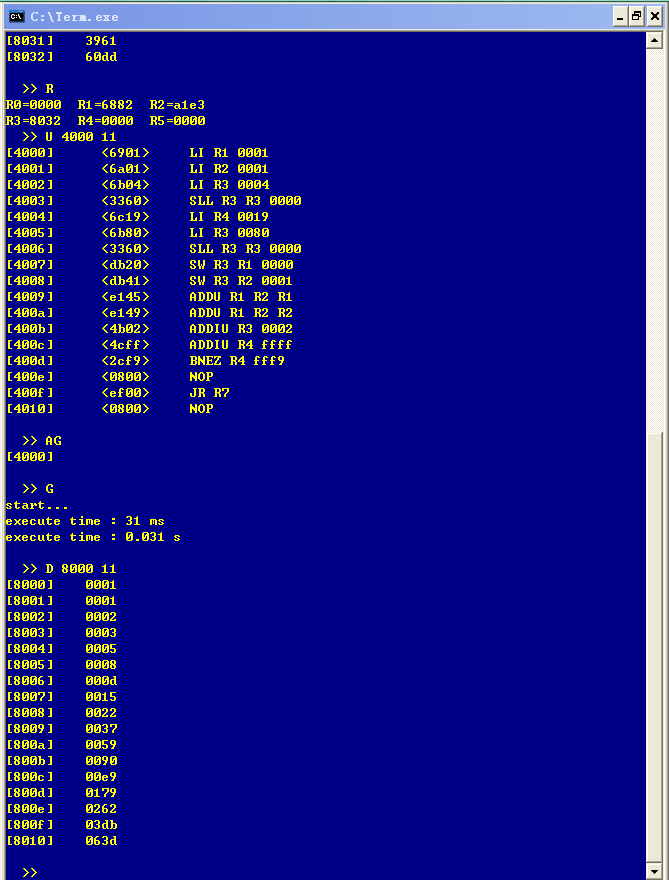
\includegraphics[width=\textwidth]{figure/result.png}
\end{figure}


\section{问题及解决}
此次实验中出现了很多问题,最后大多得以解决.
\subsection{中断}
由于设计时未想清楚,将硬中断当作跳转指令处理,而没有考虑插入时读入了一个跳转指令,导致程序出现不稳定错误.
后来在随机仿真测试中才发现该问题.
\subsection{RAM访问}
手动时钟测试没有问题之后,将CPU时钟定为50M,
发现对RAM的写入存在问题,
反复多次调试无果后, 注意到RAM的最短数据保持时间,将时钟降为25M后获得成功.
\subsection{链接错误}
曾经出现过莫名的错误,调试逻辑半天无果后打开了RTL图,
发现是已将一个调试信号输出删除,其父模块的链接表中却依然保留了该信号,使得出现在其之后的信号全部错位,修复后问题解决.

\section{经验及总结}
\subsection{仿真与调试}
  实验中调试的困难主要来源于频率低(编译时间长), 信息量少(LED, 数码管).
  因而实验中, 尽量多对代码做仿真, 以减少实际调试.
  同时, 可以提前实现VGA调试器, 以方便对CPU状态的检测, 我们在VGA上打出了CPU中几乎所有寄存器的值,
  这对我们的调试有很大帮助.

\subsection{版本控制}
我们采用git做为版本控制手段, 分为两个分支.
由于监控程序没有TLB,而且需要串口通信,与最终预期目标存在较大的冲突,因此在完成基础部分之后分裂为master和basic两个分支进行开发.
master分支实现了PS/2键盘和软硬中断以及显存的原型,而basic分支无中断,增加了串口通信,可以运行监控程序.

使用git主要是为了多人协作,同时也能够保存每个版本的信息,方便进行回滚和比较.git提交截图如下:
\begin{figure}[H]
  \centering
  \includegraphics[width=0.5\textwidth]{figure/git.png}
\end{figure}


\subsection{致谢}
计原实验的艰苦又快乐的一个月里, 我们都收获良多.
感谢刘卫东, 李山山老师及关孟翔助教在实验中给予的支持和帮助!


\end{document}
